%\setcounter{page}{1}
\setcounter{equation}{0}
\setcounter{figure}{0}

\section{Einstein Solid}

Name \rule{2.0in}{0.1pt}\hfill{}Section \rule{1.0in}{0.1pt}\hfill{}Date
\rule{1.0in}{0.1pt}

\textbf{Objective}

To develop a quantum-mechanical model of an elemental solid ({\it e.g.} aluminum) and
introduce the ideas of statistical mechanics.

\textbf{Overview of the Model}

One of the earliest successful applications of quantum mechanics was done by Albert Einstein
in 1907 when he developed a model of an elemental solid ({\it i.e.} one that consists of a single
element from the periodic table like aluminum, lead, {\it etc.}).
We start by assuming that each atom in the solid is bound in a square lattice with each
of six neighbors. Each bond is treated as a simple spring so the 
mechanical energy for a single atom is
%\begin{wrapfigure}[16]{l}{3.0in}
%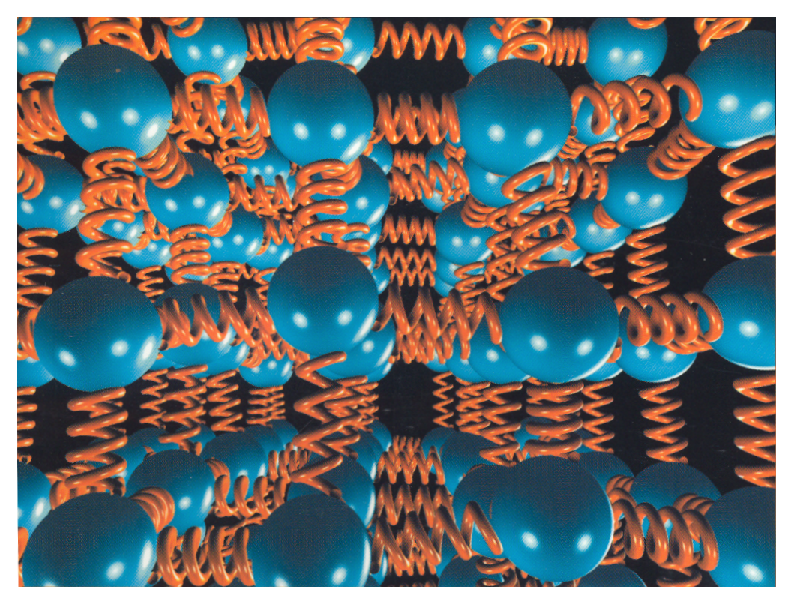
\includegraphics[height=2.0in]{EinsteinSolid/einstein_solid_picture2.eps}
%
%\hfil Fig. 1 Einstein solid.\hfil 
%
%\setcounter{figure}{1}
%
%\end{wrapfigure}
\begin{equation}
E = \frac{1}{2} m (v_x^2 + v_y^2 + v_z^2) + \frac{1}{2} k (x^2 + y^2 + z^2)
\end{equation}
where $k$ is the spring constant of the bond, the coordinates $x$, $y$, and $z$ are relative to the
equilibrium position of the atom and $v_x$, $v_y$, and $v_z$ are the components of the velocity.
Einstein used an idea pioneered by Max Planck in 1901 and
guessed the energy in the solid came in discrete pieces or quanta that were all
the same size.
Adding or removing these quanta heated or cooled the solid.
Many years later the quantum mechanical energy $E$ for a mass on a spring was found 
to be
\begin{equation}
E = (n_x + n_y + n_z + \frac{3}{2})\hbar \omega
\end{equation}
where $\hbar$ is Planck's constant, $\omega$ is related to the spring constant $k$ of the bond
mentioned
above, and $n_x$, $n_y$, and $n_z$ represent the number of quanta associated with each
degree of freedom of the spring.
The degrees of freedom here correspond to the three possible directions each atom can vibrate.
The size of each energy quantum is $\epsilon = \hbar \omega$.
The total number of energy quanta in the solid is labeled $q_A$ so the internal energy is
$E_{int} = q_A\epsilon$.
We then assume that all microstates of the solid have an equal probability of being populated.
A microstate is a specific arrangement of the quanta on the atoms in the solid.

\textbf{Activity 1: The Statistics of Matter}

Before you embark on building the model of the Einstein solid consider some ideas from
your previous study of gases. 
You will make some predictions here about the statistical nature of matter that you can
refer back to later on in this unit.

(a) Consider a gas in a container. Would it violate Newton's Laws or any other physical law
if all the particles in the gas collided in such a way that all of the gas particles
ended up in the bottom half of the container leaving the top half empty?
\vspace{15mm}

(b) Is such a scenario likely? Explain.
\vspace{15mm}

(c) If you started out with all the gas in the bottom half of the container how likely is
it to stay there?
\vspace{15mm}

The questions you answered above are addressing the notion of irreversibility.
Many processes in nature appear to proceed in one `direction' only.
When you add milk to coffee it disperses throughout the coffee.
After it is dispersed, the milk never re-concentrates into a blob of milk in the
middle of the coffee.
These processes go from a more orderly configuration (a concentrated drop of milk)
to a disordered state (milk spread throughout the liquid).
The reverse never happens.
We will return to this notion again in this laboratory.

\textbf{Activity 2: Calculating the Multiplicity of Some `Solids'}

(a) You will first calculate the configurations of 
the quanta (the microstates) for a VERY simple solid consisting of a single
atom!
The number of atoms for solid $A$ is $N_A=1$ so there are three degrees of
freedom $N_a=3$ because there is one degree of freedom for each
spatial direction.
The atom's vibration can be decomposed into three components, one for each direction.
Let the `solid' contain two quanta of energy so $q_A=2$.
Make a table with the headings $n_1$, $n_2$, and $n_3$ 
and in each row enter one
arrangement of the two quanta.
Each row in the table is a microstate.
Make a table with all of the possible microstates.
The multiplicity $\Omega_A$ of the system is the number of all possible
microstates. What is your multiplicity?
Record it here.
\vspace{45mm}

(b) You can calculate the multiplicity $\Omega_A$ using the expression
\begin{equation}
\Omega(N_A,q_A) = \frac{(q_A + 3N_A -1)!}{q_A! (3N_A-1)!}
\end{equation}
Make the calculation for $N_A = 1$ and $q_A = 2$.
Does this agree with your result in part 2.a?
\vspace{15mm}

(c) Now do the same thing for a different `solid'.
This time for solid $B$, let $N_B = 2$ (two whole atoms!) and $q_B = 1$.
How many degrees of freedom does solid $B$ have?
Make a table analogous to the one in part 2.a on the same sheet as before.
What is the multiplicity of solid $B$?
Record it here.
Use the expression in Activity 2.b to check your calculation.
\vspace{45mm}

\textbf{Activity 3: Putting the `Solids' Together}

When two solids are brought together heat/energy can flow between the two objects.
For the model of the Einstein solid you are building this corresponds to 
energy quanta ($\hbar \omega$) moving from atom to atom and occupying different
microstates of the combined system.

(a) Now bring the your solids $A$ and $B$ `together' into a single system.
What is $N_{AB}$ the total number of atoms?
What is the number of degrees of freedom of the combined system?
\vspace{10mm}

(b) What is the total number of energy quanta $q_{AB}$ for the combined system?
\vspace{10mm}

(c) The system is in its initial macrostate.
A macrostate is a configuration of the system defined here by the total number
of atoms and quanta in each solid.
In this case the macrostate is defined by $N_A=1$, $q_A=2$, $N_B=2$, and $q_B= 1$.
 What is the total multiplicity $\Omega_{AB}$ for the combined system
with $q_A=2$ and $q_B=1$ in its initial macrostate?
\vspace{15mm}

(d) Now take the energy quantum in solid $B$ and put it in solid $A$,
{\it i.e.}, let heat flow from solid $B$ into solid $A$.
This is now a macrostate where $q_A=3$ and $q_B=0$.
What is the new multiplicity $\Omega_A$ for solid $A$ and the  multiplicity $\Omega_B$ for solid $B$?
\vspace{20mm}

(e) What is the multiplicity $\Omega_{AB}$ for the combined system (solids $A$ and $B$)?
\vspace{15mm}

(f) Remember that a macrostate is defined by the combination of $N_A$, $N_B$, $q_A$, and $q_B$.
Which macrostate had the greatest multiplicity, $(q_A=2, ~ q_B=1)$ or $(q_A=3, ~ q_B=0)$
(remember that $N_A$ and $N_B$ are the same in each configuration so we don't 
list those parameters here)?
\vspace{15mm}

(g) If the energy quanta can move from atom to atom
which macrostate $(q_A=2, ~ q_B=1)$ or $(q_A=3, ~ q_B=0)$ is most probable? Why?
\vspace{15mm}

(h) If you started out in the $(q_A=3, ~ q_B=0)$ macrostate is it more likely that you will remain
in that macrostate of evolve to the $(q_A=2, ~ q_B=1)$ macrostate? Why?
\vspace{15mm}

What you have discovered is a version of the irreversibility mentioned earlier,
One macrostate ($q_A=2$, $q_B=1$) is preferred over the other because it has more microstates
than the other.
This result depends critically on your assumption that all states are equally populated.

\newpage

\textbf{Activity 4: Using {\it StatMech} For More Complex Cases}

You should have found in the previous activity that the $(q_A=2, ~ q_B=1)$ 
macrostate was more likely
to occur and the process proposed in part 3.d is relatively unlikely.
In other words, it is more likely for energy to be spread evenly throughout the system.
This is good news because it means the statistical picture we are painting is consistent
with reality.
Remember what happens to the blob of milk in the coffee.

(a) You should realize that making the sorts of calculations you did in Activity 3 above would
become rather painful for say $N_A = 300$ atoms.
In order to push the model further you will use a software packaged called 
{\it StatMech} to perform the same calculations.
To run the program go to the {\tt Physics Applications} menu and click on
{\tt StatMech}.
You should see a window like the one below.
\begin{figure}[h!]
\begin{center}
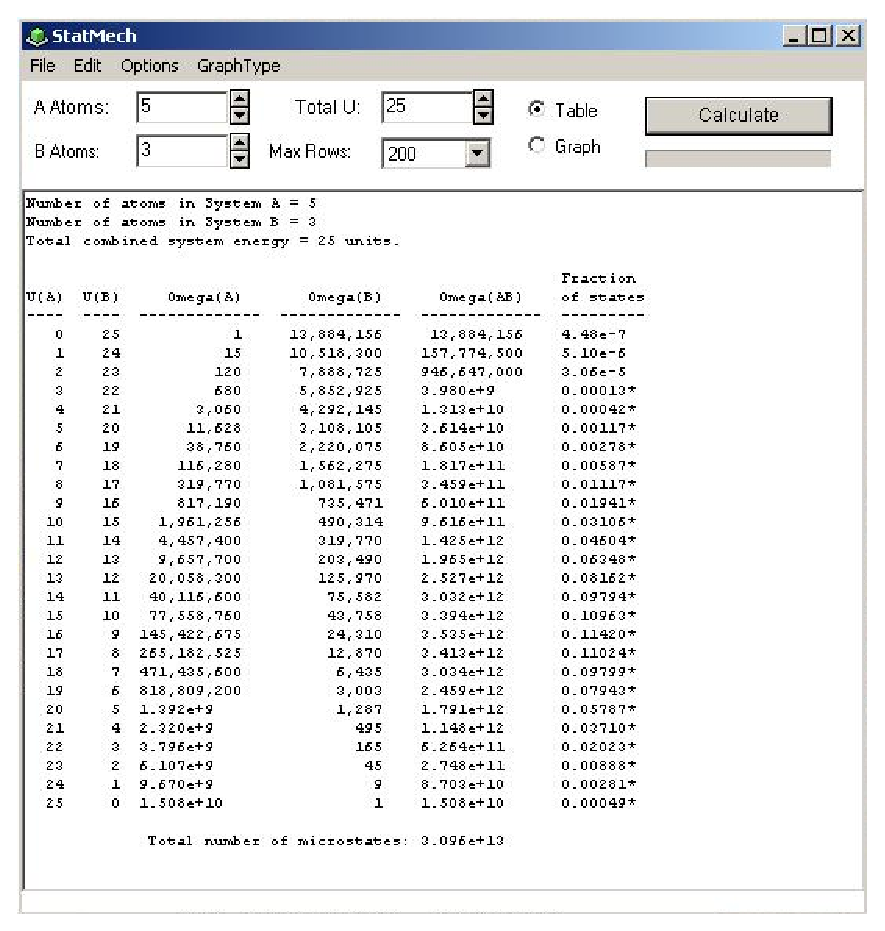
\includegraphics[height=4.0in]{EinsteinSolid/statmech1.eps}
\caption{The {\tt StatMech} window showing the table of multiplicities for each microstate.
Each row corresponds to a different value of $q_A$.}
\end{center}
\end{figure}
The top of the window has several entry boxes where you can set the number of
atoms ($N_A$ and $N_B$) and the total number of energy quanta in the system $U$.
The parameter $U$ is the total internal energy $_{int}$ in the system in 
units of $\epsilon = \hbar \omega$.
It is equivalent to the sum $q_{AB} = q_A + q_B$.
You can also set the number of rows of microstates to print out
or choose to view a graph instead of the table.
To test the operation of {\it StatMech} redo the calculations of the microstates that
you did in Activity 3. Make sure your results in Activity 3 agree with the output of 
{\it StatMech}.
You will also see there are other macrostates that were ignored in Activity 3 for
simplicity.

(b) Now run {\it StatMech} for the case where $N_A = 10$, $N_B=20$, $U = 500$.
What is the value of $q_A$ for the most probable macrostate? 
%qA = 165.
Record it here.
Click on the button at the top of the {\it StatMech} window and choose graph.
You will see a graph of the table  and it should look something like
Figure 2.
\begin{figure}[h!]
\begin{center}
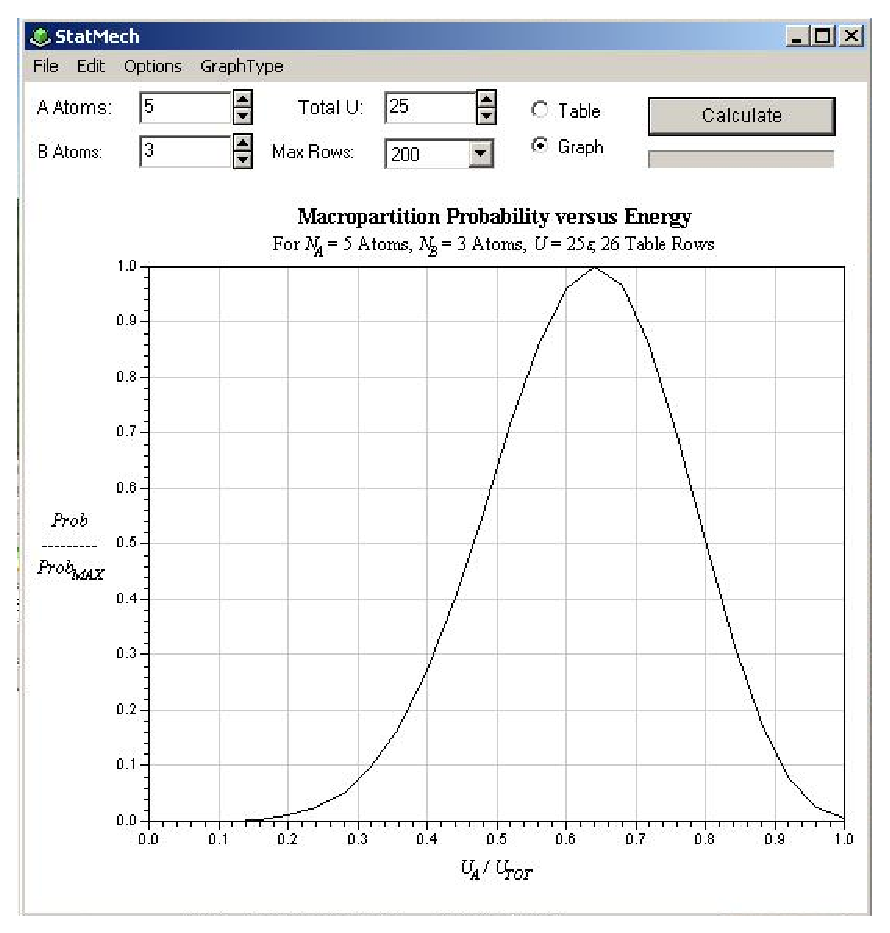
\includegraphics[height=4.0in]{EinsteinSolid/statmech2.eps}
\caption{The {\tt StatMech} window showing a graph of the multiplicities as a function
of $E_A/E_{int}$ where $E_A = q_A \hbar \omega$ and 
$E_{int} = q_{AB} \hbar \omega = (q_A+q_B)\hbar \omega$.}
\end{center}
\end{figure}
The vertical axis is the probability of a particular macrostate divided by the maximum
probability of any macrostate.
The horizontal axis is  $U_A/U_{TOT}$ where 
$U_A$ is the energy of solid $A$ in units of $\epsilon$ (equivalent to $q_A$) and $U_{TOT}$ is the total
internal energy of the solid in units of $\epsilon$ (equivalent 
to the total number of quanta $q_{AB}$).
What is the value of $U_A/U_{TOT}$ for the most probable state?
How is this value related to the value of $q_A$ for the most probable macrostate? 
Also, explain in words what this plot is showing you.
\vspace{25mm}

(c) How wide is the distribution of microstates?
Measure this number by estimating the full-width-half-maximum (FWHM) from your graph.
Do this by finding the largest value on the vertical axis, divide that value by two, and find
the two points on either side of the peak where the distribution is equal to that
half-maximum.
Take the difference between these two points along the horizontal and this is the FWHM.
Record your result here.
%$U_A/U_{TOT} = 0.32
% sigma = 0.39-0.26 = 0.13
\vspace{15mm}

(d) Now repeat steps 4.b-c with $U=100,000$ and $N_A$ and $N_B$ at their last values.
What is the most probable value of $U_A/U_{TOT}$ and the FWHM?
How have things changed?
%$E_A/U_{TOT} = 0.32
% sigma = 0.39-0.26 = 0.13
\vspace{15mm}

\newpage

(e) Keeping $U=100,000$ now repeat steps 4.b-c, but this time double the values of $N_A$ and $N_B$.
Record the most probable macrostate and the FWHM.
Repeat this doubling of the number of atoms in each solid while keeping $U$ fixed at least 3-4 times.
Record the most probable macrostate and the FWHM each time along with $N_A$ and $N_B$.
% 10:20 peak=0.32 sigma=0.13
% 20:40 peak=0.32 sigma=0.38-0.29=0.09
% 40:80 peak=0.32 sigma=0.36-0.30=0.06
% 80:160 peak=0.32 sigma=0.35-0.31=0.04
% 160:320 peak=0.32 sigma=0.34-0.32=0.02
\vspace{45mm}

(f) How does the value of $q_A$ for the most probable macrostate change as the number
of atoms increases?
\vspace{15mm}

(g) How does the FWHM change as the number of atoms increases?
\vspace{15mm}

\textbf{Activity 5: Irreversibility}

You will now use the results from the previous Activity to delve into some of the
implications of the statistical mechanics of the Einstein solid.

(a) As the number of atoms increases, what happens to the probability for finding the
system in a macrostate different from the most probable one?
Use the results of your calculations to explain your answer.
\vspace{15mm}

(b) When the system is in a macrostate far from the most probable one, what is the most
likely thing to happen as energy or heat flows around the system?
\vspace{15mm}

(c) For the last calculation in Activity 4 
what is the probability of the state with the minimum value of $q_A$?
%10^-813
In other words what is the probability that all of the quanta would end up all in solid $B$?
What is the probability of the most probable macrostate?
%qA=334, frac = 0.03186
\vspace{15mm}

(d) Go back to the questions in Activity 1 and look at your answers. 
Do they still appear to be correct?
A situation where all of the gas particles end up in one part of the container is a macrostate
of the system analogous
to the situation in Activity 5.c where all of the quanta end up in one  of the solids and 
not the other.
Answer those questions in Activity 1 again in terms of microstates, macrostates, and probability.

The behavior you are seeing here is for an Einstein solid, but is actually typical for
most macroscopic systems. These systems have a large number of atoms or molecules
with a variety of different energy states available.
They evolve to the most probable macrostate and there is essentially no chance to occupy a state
far from the most probable one. 
When two materials are first put in thermal contact they may be far from the most probable 
macrostate, but they equilibrate at that most probable one (where the temperatures are equal)
and never go back.
This is irreversibility.

\vspace{15mm}


\bigskip

\textbf{Activity 6: Homework Problems} (E - exercise, P - problem)

\begin{enumerate}

\item(E) Consider the following `gas'.
It consists of four atoms in a cubical box. At any instant, there is a 50\% chance
of each atom being in the left half of the box ($L$) or the right half ($R$).
Make a table showing all the microstates of this system. (Hint: There are 16.)
How many macrostates are there?
How many microstates are in each macrostate?

\item (E) Show that for $N$ gas atoms in a box, the number of possible microstates is
$2^N$ when microstates are defined by whether a given molecule is in the left half
of the box or the right half of the box.
The volumes of each half are equal.


\item (E) Imagine that we have an ideal gas consisting of 15 molecules.  
We can flip the signs of each of the three velocity components of a given molecule w
without changing its overall energy (and thus without changing the gas's macrostate).  
How many possible patterns of sign choices are there?

\item (E) Calculate the multiplicity of an Einstein solid with $N = 1$ and $E_{int} = 6\epsilon$ 
by directly listing and counting the microstates.  
Check your work by using equation 3.

\item (E) Calculate the multiplicity of an Einstein solid with $N = 1$ and 
$E_{int} = 5\epsilon$  by directly listing and counting the microstates.  
Check your work by using equation 3.

\item (E) Use equation 3 to calculate the multiplicity of an 
Einstein solid with $N = 4$ and $E_{int} = 10\epsilon$.

\item (E) Use equation 3 to calculate the multiplicity of an 
Einstein solid with $N = 3$ and $E_{int} = 15\epsilon$.

\item (E) How many times more likely is that the combined system of 
solids described in the table below will be found in macropartition 3:3 than 
in macropartition 0:6, if the fundamental assumption is true?

\item (E) How many times more likely is it that the combined system of 
solids describe in the table below will not be found in macropartition 3:3 
than it is to be found in macropartition 0:6, if the fundamental assumption is true?

\begin{table}[h!]
\begin{center}
\begin{tabular}{|lccccc|} \hline
\hi Macropartition  & $E_A$ & $E_B$ & $\Omega_A$ & $\Omega_B$ & $\Omega_{AB}$ \\[5pt] \hline
\hi 0:6             & 0     & 6     & 1          & 28         & 28            \\[5pt]
\hi 1:5             & 1     & 5     & 3          & 21         & 63            \\[5pt]
\hi 2:4             & 2     & 4     & 6          & 15         & 90            \\[5pt]
\hi 3:3             & 3     & 3     & 10         & 10         & 100            \\[5pt]
\hi 4:2             & 4     & 2     & 15         & 6          & 90           \\[5pt]
\hi 5:1             & 5     & 1     & 21         & 3          & 63            \\[5pt]
\hi 6:0             & 6     & 9     & 28         & 1          & 28           \\[5pt] \hline
\hi                 &       &       &            & Total=     & 462         \\[5pt] \hline
\end{tabular}
\end{center}
\caption{Possible macropartitions for $N_A=1$, $N_B=1$, $E_{int}=6\epsilon$.}
\end{table}

\item (E) Consider the system consisting of a pair of Einstein solids in thermal contact.  
A certain macropartition has a multiplicity of $3.7 \times 10^{1024}$, while the total number of 
microstates available to the system in all macropartitions is $5.9 \times 10^{1042}$.  If we look 
at the system at a given instant of time, what is the probability that we will find it 
to be in our certain macropartition?

\item (E) Consider the system consisting of a pair of Einstein solids in thermal contact.  
A certain macropartition has a multiplicity of $1.2\times 10^{346}$, while the total number of 
microstates available to the system in all macropartitions is $5.9 \times 10^{362}$.  If we look 
at the system at a given instant of time, what is the probability that we will find it 
to be in our certain macropartition?

\item (E) Consider the system consisting of a pair of Einstein solids in thermal contact.  
Imagine that it is initially in a macropartition that has a multiplicity of $8.8 \times 10^{123}$.  
The adjacent macrostate closer to the equilibrium macrostate has a multiplicity
of $4.2 \times 10^{1234}$.  If we look at the system a 
short later, how many times more likely is it to have moved to the second macropartition 
than to have stayed with the first?

\item (E) Consider the system consisting of a pair of Einstein solids in thermal contact.  
Imagine that it is initially in a macropartition that has a multiplicity of $7.6 \times 10^{3235}$.  
The adjacent macropartition closer to the equilibrium macropartition has a multiplicity 
of $4.1 \times 10^{3278}$.  If we look at the system a short time later, how many times more likely 
is it to have moved to the second macropartition than to have stayed with the first?

\item(P) Suppose you put 100 pennies in a cup, shake it up, and toss them all into the
air.
(a) After landing, how many different head-tail arrangements (microstates) are possible for
the hundred pennies?
(b) What is the probability of finding exactly 50 heads? 
(c) 49 heads?
(d) 1 head?

\item(P) You ask your roommate to clean up a mess he or she made in your room.  Your roommate 
refuses, because cleaning up the mess would violate the second law of thermodynamics, and 
campus security's record of your roommate's legal violation is already excessive.  
Gently but firmly explain why complying will not put your roommate at risk of such an infraction.

\item(P) The classic statement of Murphy's law reads, `If something can go wrong, it will.'   
Explain how this is really a consequence of the second law of thermodynamics.  (Hint:  
What is the entropy of `wrong' in a given context compared to the entropy of `right'?)

\item(P) Run the {\it StatMech} program to answer the questions below.

\begin{enumerate}

\item For two Einstein solids in contact with 
$N_A = N_B = 100$ and 
$E_{int} = 200\epsilon$ answer the following questions.  (1) How many times more likely is the system 
to be found in the center macropartition than in the extreme macropartition where $E_A = 0$ 
and $E_B = 200\epsilon$ 
(2) What is the range of values that $E_A$ is likely to have more than 99.98\% 
of the time?  (3) if $E_A$ were initially to have the extreme value 0, how many times more 
likely is it to move to the next macropartition nearer the center than to remain in the 
extreme one?
\item  Answer the same question as in (a) for a run where you scale everything up by a 
factor of 10, so that $N_A = N_B = 1000$ and $E_{int} = 2000\epsilon$.
\item  Answer the same question as in (a) for a run where $N_A = N_B = 1000$ and 
$E_{int} = 200\epsilon$.  
Comment on the effect that increasing just the size of the system by a factor of 10 
has on these answers.
\item Answer the same question as in (a) for a run where $N_A = N_B = 100$ and $E_{int} = 2000\epsilon$.  
Comment on the effect that increasing just the energy available to the system by a factor 
of 10 has on these answers.

\end{enumerate}

\item(P) Consider two Einstein solids in thermal contact.  The solids have different 
values of N but are identical in all other respects.  It is plausible, since every atom 
in the combined system is identical, that in equilibrium the energy will be distributed 
among the solids in such a way that the average energy per atom is the same.  Use {\it StatMech} 
to test this hypothesis in the situation where $E_{int} = 1000\epsilon$ and $N_A$ and $N_B$ have various 
different values such that $N_A + N_B = 1000$.  (Set {\tt Max Rows} to 1000 so that you can see 
every macropartition).
\begin{enumerate}
\item Is it true in most cases that in the most probable macropartition the solids have 
energies such that the average energy per atom in each is the same?  Is it strictly 
true in every case?  Answer these questions by discussing the values $N_A$ and $N_B$ you tested, 
and whether the actual most probable macropartition is the same as that predicted by the hypothesis.
\item In any case where the hypothesis does not work, does increasing both $N_A$ and $N_B$ by a 
factor of 10 or 100 (but leaving $U$ alone) yield a result more or less consistent with 
the hypothesis?
\item Speculate as to the value of this hypothesis in the large-$N$ limit.
\end{enumerate}
\item(P) For the following questions, you will find that using {\it StatMech} is 
by far the fastest way to calculate the multiplicity.
\begin{enumerate}
\item  What is the entropy of an Einstein solid with 5 atoms and an energy of 
$15\epsilon$?  Express your answer as a multiple of $k_b$.
\item  What is the entropy of an Einstein solid with 50 atoms and an energy of $100\epsilon$?  
Express your answer as a multiple of $k_b$.
\end{enumerate}

\item(P) A certain macropartition of two Einstein solids has an entropy of $305.2k_b$.  
The next macropartition closer to the most probable one has an entropy of $335.5k_b$.  
If the system is initially in the first macropartition and we check it again later, 
how many times more likely is it to have moved to the other than to have stayed in the first?

\item(P) My calculator cannot display $e^x$ for $x> 230$.  One can calculate $e^x$ for larger 
values of $x$ as follows.  Define $y$ such that $x = y \ln 10$.  This means that 
$e^x = e^{y\ln 10} = (e^{\ln10})^y = 10^y = 10^{x\ln 10}$.  
Note that we can calculate 10 raised to a 
non-integer power (for example, 103.46) as follows:  
$10^{3.46} = 10^{3+0.46} = 10^3(10^{0.46}) = 2.9 \times 10^3$.  
Use these techniques to solve the following problem.  The entropy of the most probably 
macropartition for a certain system of Einstein solids is $6025.3k_b$, while the entropy 
of an extreme macropartition is only $5755.4k_b$.  What is the probability of finding the 
system at a given time in the extreme macropartition compared to that of finding it in 
the most probable macropartition?

\item(P) In principle, the entropy of a isolated system decreases a little bit whenever 
random processes cause its macropartition to fluctuate away from the most probable 
macropartition.  We can certainly see this with small systems. 
But is this really a possibility for a typical macroscopic system?  Imagine that 
we can measure the entropy of a system of two solids to within 2 parts in 1 billion.  
This means that we could just barely distinguish a system that has an entropy of 
4.99999999 J/K (eight 9s!) from one that has 5.00000000 J/K.  (This is a reasonable 
entropy for a macroscopic system).
\begin{enumerate}
\item Imagine that the entropy of the equilibrium macropartition is 5.00000000 J/K.  
Show that the approximate probability that at any given time later we will find the 
system in a macropartition with entropy 4.99999999 J/K ({\it i.e.}, with an entropy that 
is only barely measurably smaller) is about 10315,000,000,000,000 times smaller that 
the probability we will still find it to have entropy 5.00000000 J/K. (Hint:  See problem 17.)
\item Defend the statement that the entropy of an isolated system in thermal equilibrium 
never decreases.
\end{enumerate}

\end{enumerate}



